\section{Quality Assurance}

\begin{frame}[fragile] {Quality Assurance} {Fulfilling the semester description}
	\begin{itemize}
		\item Quality assurance (in terms of program testing and results and usability evaluation and results), including arguments for coverage and validity {\footnotesize (Semester description)}
		\begin{itemize}
			\item Program testing = Unit testing
			\item Usability evaluation = Instant Data Analysis (report chapter 11)
		\end{itemize}				
	\end{itemize}

\end{frame}

\subsection{Unit Testing}

\begin{frame}[fragile] {Unit Testing} {What is unit testing?}
	\begin{itemize}
		\item Initial stage of program testing
		\item Isolate smallest testable code
		\item Confirm if the unit behaves correctly
	\end{itemize}
\end{frame}

\begin{frame}[fragile] {Unit Testing} {Possible candidates for unit testing}

	\begin{itemize}
		\item Classes e.g. User, Ingredient or Recipe
			\begin{itemize}
				\item Testing their properties or methods
			\end{itemize}
		\item List of candidates	 	
				{\small
				\begin{tabular} {l r}
							\textbf{Models} & \textbf{ViewModels} \\
							Graylist & {\color{blue} InventoryViewModel} \\
							Ingredient & MealPlanViewModel \\
							{\color{blue}InventoryIngredient} & RecipeSearchViewModel \\
							InventoryListCombinedByQuantity & RecipeViewModel \\
							LastMeal & SettingsViewModel \\
							PublicQuerys & ShoppingListViewModel \\
							Recipe \\
							RecipeIngredient \\
							SearchResults \\
							ShoppingClass \\
							ShoppingListIngredient \\
							User
				\end{tabular}
				}					
	\end{itemize}
		
\end{frame}

\begin{frame}[fragile] {Unit Testing} {Code from InventoryIngredientTests.cs}
		
\begin{lstlisting}
[TestMethod]
public void PurchaseDate_AutoSetConstructor_SetToNow() {
  //arrange
  Ingredient testIngredient = new Ingredient();
  DateTime expectedPurchaseDate = DateTime.Now;

  //act - The property is set automaticly in the constructor
  InventoryIngredient testInventoryIngredient = new InventoryIngredient(testIngredient, 750);
  //assert
  Assert.AreEqual(expectedPurchaseDate, testInventoryIngredient.PurchaseDate); 
}
\end{lstlisting}
	
\end{frame}

\begin{frame} [fragile] {Unit Testing} {Code from InventoryViewModelTests.cs}

\begin{lstlisting} []
[TestMethod]
public void
AddInventoryIngredient_CorrectIngrAdded_InventoryUpdated() {
  //arrange
  Ingredient expectedNewIngredient = new Ingredient();
  InventoryIngredient inventoryIngredient = new InventoryIngredient (expectedNewIngredient, 1);
  InventoryViewModel inventoryViewModel = new InventoryViewModel();
  bool ingredientAdded = false;
  
  //act
  inventoryViewModel
    .AddIngredientToInventory(expectedNewIngredient, 1);
  
  if (FoodPlanner.App.CurrentUser
      .InventoryIngredients.Contains(InventoryIngredient)) {
    ingredientAdded = true;
  }
    
  //assert
  Assert.IsTrue(ingredientAdded);
}
\end{lstlisting}

\end{frame}

\begin{frame} {Unit Testing} {Dependency injection}

Current dependency (tight coupling) \newline

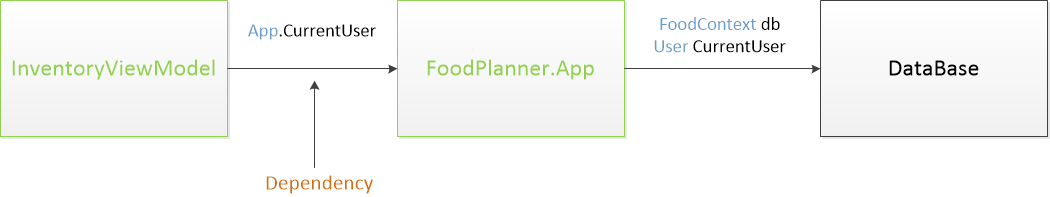
\includegraphics[width = \textwidth] {graphics/currentDependency.png}
%første pil uses og sidste fetches data from db
\end{frame}

\begin{frame} {Unit Testing} {Dependency injection}
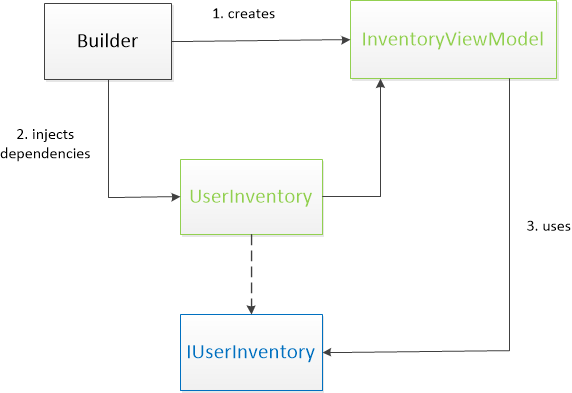
\includegraphics[width = \textwidth]{graphics/dependencyInjectionBasic.png}
\end{frame}


\begin{frame} [fragile] {Unit Testing} {Dependency injection}

\begin{lstlisting}
public interface IUserInventory {
  public void FecthUserInventory();
}
\end{lstlisting}

\begin{lstlisting}
public class UserInventory : IUserInventory {
  public void FetchUserInventory() {
    //Go to db and fetch the user's inventory
  }
}
\end{lstlisting}

\begin{lstlisting}
public class InventoryViewModel {
  private IUserInventory _userInventory;
  
  public InventoryViewModel(IUserInventory userInventory) {
    this._userInventory = userInventory;
  }
  
  public void Start() {
    this._userInventory.FetchUserInventory();
    //User inventory fetched and ready for use
  }
\end{lstlisting}

\begin{lstlisting}
InventoryViewModel inventoryViewModel = new InventoryViewModel(new UserInventory();

inventoryViewModel.Start();
\end{lstlisting}

\end{frame}

\begin{frame} {Unit Testing} {Dependency injection}

\begin{itemize}
	\item issues
		\begin{itemize}
			\item it is hard coded
			\item instantiating is custom
		\end{itemize}
\end{itemize}

\begin{itemize}
	\item Using Locators
		\begin{itemize}
			\item map of dependencies
			\item logic to create the dependencies
		\end{itemize}
	\item New class(); -> Locater -> return class
	\item Using dependency frameworks e.g. Ninject 
\end{itemize}

\end{frame}